\chapter{Introdução}

\section{História da Genética}

\indent O estudo do núcleo celular começou no século XIX, em um laboratório na Alemanha, com o objetivo de catalogar as substâncias químicas presentes nas células sanguíneas do ser humano. Como naquela época as pesquisas eram mais voltadas ao citoplasma - fluido pastoso que constitui a célula, o bioquímico suíço Friedrich Miescher foi o pioneiro no estudo do núcleo. Ele quem descobriu a substância nucleína composta por carbono, hidrogênio, oxigênio, nitrogênio e fósforo (ausênte nas proteínas), que mais tarde chamaram de ácido desoxirribonucléico, ou DNA. \\

\indent No início do século XX, o geneticista estadunidense Thomas Morgan liderou uma equipe de estudantes e realizou vários experimentos em \textit{Drosophila melanogaster} - espécie de mosca, com a finalidade de compreender a hereditariedade a partir de genes transmitidos aos organismos em desenvolvimento. Esta pesquisa foi fundamental para demonstrar exerimentalmente a Teoria Cromossômica da Hereditariedade (Sutton-Boveri, 1902), que assumem várias suposições como verdade, dentre elas: Os genes estão localizados em cromossomos; Os cromossomos formam pares de homólogos; Destes pares, um tem origem paterna, o outro tem origem materna. Tais hipóteses são baseadas nos experimentos caseiros do botânico Gregor Mendel, que após 8 anos de experimentos (1856-1863), publicou seu paper na Nature Research Society of Brünn. Nele, Mendel introduz conceitos como dominância, fator recessivo, hereditariedade, segregação dos fatores e transmissão independente dos genes. O trabalho de Morgan e sua equipe rendeu-lhe um Prêmio Nobel de Fisiologia ou Medicina em 1933. \\

\indent No início dos anos 50, uma química britânica chamada Rosalind Frankling usou a técnica de difração de raios-X para determinação da estrutura da biomolécula do DNA e concluiu que sua forma era helicoidal. Seu trabalho foi empregado nos experimentos de dois pesquisadores, Francis Crick e James Watson, em um laboratório em Cambridge, na Inglaterra. No mesmo ano, a dupla decifrou a estrutura do DNA: duas longas fitas enroladas uma na outra em espiral para a direita, ligadas por pares de bases complementares, formando o que chamaram de dupla-hélice. Apesar da grande descoberta, isto não era o suficiente para entender como eram produzidas as proteínas, portanto os cientistas mudaram o foco das pesquisas para o RNA, uma vez que sabiam o quanto sua concentração aumentava sempre que as células começavam a produzir proteínas. Em 1958, Crick e Watson anunciaram mais uma descoberta: A partir do DNA, o processo de \textit{transcrição} fornece uma fita de RNA, que por sua vez, a partir do processo de \textit{tradução}, fornecem a proteína. Esta sequência de processos ficou conhecida como Dogma Central da biologia molecular. \\

\textbf{CITAR: O polegar do violinista}

\vspace{1cm}
 \begin{figure}[h!]
     \centering
     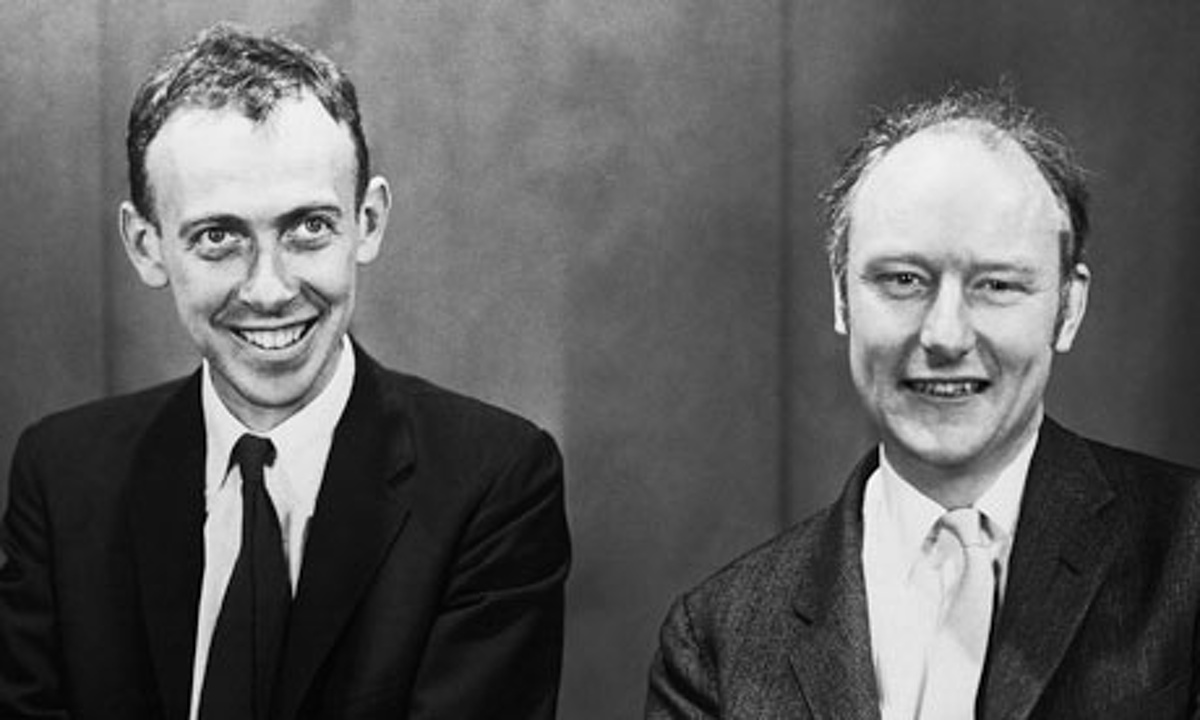
\includegraphics[scale=0.4]{JamesWatsonAndFrancisCrick.jpg}
     \caption{James Watson e Francis Crick}
     \label{fig:JamesWatsonAndFrancisCrick}
 \end{figure}
\vspace{1cm}

\indent Bioinformática. Margaret Dayhoff e Walter Goad \\.\\.\\.\\.\\.\\.\\.\\

%  -------------------------------------------------------------
%  -------------------------------------------------------------

\indent A linha do tempo abaixo tem o objetivo de auxiliar na localização temporal da história da biologia molecular e da bioinformática ao passo que apresentam as datas de nascimento dos principais pesquisadores da área.

%  -------------------------------------------- 
%  -------------------------------------------- LINHA DO TEMPO
%  -------------------------------------------- 

\begin{timeline}{1809}{1933}{2cm}{2.5cm}{10cm}{1\textheight}
\entry{1809}{$\star$ Charles Darwin, Inglaterra}
\entry{1822}{$\star$ Gregor Mendel, Áustria}
\entry{1844}{$\star$ Friedrich Miescher, Suíça}
\entry{1859}{Darwin publica livro A Origem das Espécies} %On the Origin of Species by Means of Natural Selection,
% or the Preservation of Favoured Races in the Struggle for Life.
%  6º ed. It is in this edition that the word 'evolution' occurs for the first time.
% http://darwin-online.org.uk/content/frameset?pageseq=80&itemID=A1&viewtype=text
% Genes sobreviventes demoram a se espalhar pois são aleatóriamente selecionados
\entry{1865}{Mendel apresenta pela primeira vez seu trabalho com ervilhas}
% http://www.wired.com/2010/02/0208gregor-mendel-reads-paper/
\entry{1866}{$\star$ Thomas Morgan, Estados Unidos}
\entry{1871}{Miescher publicou seu paper sobre a nucleína}
%\entry{1882}{$\dagger$ Charles Darwin}
%\entry{1884}{$\dagger$ Gregor Mendel}
\entry{1890}{$\star$ Hermann Muller, Estados Unidos}
%\entry{1895}{$\dagger$ Friedrich Miescher} %%
\entry{1916}{$\star$ Francis Crick, Inglaterra}
\entry{1925}{$\star$ Margaret Dayhoff, Estados Unidos}
\entry{1925}{$\star$ Walter Goad, Estados Unidos}
\entry{1928}{$\star$ James Watson, Estados Unidos}
\entry{1933}{Thomas Morgan recebe Prêmio Nobel de Fisiologia ou Medicina por mostrar experimentalmente a Teoria Cromossômica da Hereditariedade}
%\entry{1945}{$\dagger$ Thomas Morgan}
%\entry{1967}{$\dagger$ Hermann Muller}
%\entry{2004}{$\dagger$ Francis Crick}
\end{timeline}


% ADICIONAR DADOS: http://www.ncbi.nlm.nih.gov/pmc/articles/PMC2898077/figure/F2/

%  -------------------------------------------- 
%  -------------------------------------------- LINHA DO TEMPO
%  -------------------------------------------- 


\section{Definição do Problema}

\indent 
Contruir uma visualização interativa de redes metabólicas aramazenadas em banco de dados de grafos que permita ao pesquisador explorar os aspectos biológicos do organismo estudado.



\section{Justificativa}

\indent 
% Falar da quantidade de dados que e muito grande para ser examinada e o quanto um sistema com busca e uma visualizacao interativa
% pode auxiliar o pesquisador.

Atualmente, a quantidade de dados <<<<>>>> estudados pelos pesquisadores é extensa e complexa. Uma maneira de amenizar o esforço feito para analisá-los e compreendê-los é oferecer uma ferramenta que aproxime o usuário (pesquisador) e os dados em forma de grafo(redes metabólicas). Esta ferramenta deverá permitir que o usuário visualize e interaja com os dados dinamicamente, além de disponibilizar mecanismos de busca em grafos, úteis para sua pesquisa.


\section{Objetivo}

\indent 
Constrir um sistema que acesse redes metabólicas armazenadas em bancos de dados em grafo e gere uma visualização interativa
\begin{itemize}
 \item Implementar uma busca das vias metabólicas de interesse a apartir de parâmetros informados pelo pesquisador no sistema
 \item Recuperar a informação desejada e exibí-la para o pesquisador de forma ergonômica
 \item Implementar algoritmos de busca em grafos para recuperar a informação solicitada e/ou sugerir informação relevante
\end{itemize}

\section{Descrição dos Capítulos}

\indent No Capítulo 1 fez-se uma breve introdução à história da biologia molecular e da bioinformática. No Capítulo 2 são estabelecidas as principais definições utilizadas neste trabalho mais profundamente, tais como ácidos nucléidos, biomoléculas gerais que originam o DNA e o RNA; a proteína, macromolécula extensa, formada por um processo complexo chamado síntese de proteína; código genético, listagem do arranjo de bases nitrogenadas que formam aminoácidos, que por sua vez compõem a proteína; Neste capítulo também são descritos os processos de sequenciamento de proteínas, na subseção de bioinformática e os desafios enfrentados nessa área. \\

\indent O Capítulo 3 apresenta uma estrutura chamada Redes metabólicas, estrutura de dados extremamente complexas que existem para auxiliar o pesquisador biólogo a entender reações intracelulares, bem como determinar propriedades fisiológicas e bioquímicas das células. A construção destas redes é possível pos existe sequenciamento do genoma do organismo estudado. O Capítulo 4 propõe um banco de dados não relacional (NoDB) em grafos como maneira de armazenar estas redes metabólicas. Nele é descrito todo o conceito de NoDB, e é apresentado aquele utilizado neste trabalho: banco de dados neo4j. \\

\indent No Capítulo 5 são exibidos os resultados da implementação do programa e no Capítulo 6, as conclusões tiradas a parir da análise dos dados. O Capítulo 7 expõe os problemas enfrentados, bem como sugestões de melhorias e trabalhos futuros. Por fim, o Capítulo 8 apresenta uma tabela do cronograma da execução deste trabalho.






